\documentclass[]{exam}
\usepackage{lmodern}
\usepackage{amssymb,amsmath}
\usepackage{ifxetex,ifluatex}
\usepackage{fixltx2e} % provides \textsubscript
\ifnum 0\ifxetex 1\fi\ifluatex 1\fi=0 % if pdftex
  \usepackage[T1]{fontenc}
  \usepackage[utf8]{inputenc}
\else % if luatex or xelatex
  \ifxetex
    \usepackage{mathspec}
    \makeatletter % undo the wrong changes made by mathspec
    \let\RequirePackage\original@RequirePackage
    \let\usepackage\RequirePackage
    \makeatother
  \else
    \usepackage{fontspec}
  \fi
  \defaultfontfeatures{Ligatures=TeX,Scale=MatchLowercase}
\fi
% use upquote if available, for straight quotes in verbatim environments
\IfFileExists{upquote.sty}{\usepackage{upquote}}{}
% use microtype if available
\IfFileExists{microtype.sty}{%
\usepackage{microtype}
\UseMicrotypeSet[protrusion]{basicmath} % disable protrusion for tt fonts
}{}
\usepackage{hyperref}
\hypersetup{unicode=true,
            pdftitle={Homework 3},
            pdfborder={0 0 0},
            breaklinks=true}
\urlstyle{same}  % don't use monospace font for urls
\IfFileExists{parskip.sty}{%
\usepackage{parskip}
}{% else
\setlength{\parindent}{0pt}
\setlength{\parskip}{6pt plus 2pt minus 1pt}
}
\setlength{\emergencystretch}{3em}  % prevent overfull lines
\providecommand{\tightlist}{%
  \setlength{\itemsep}{0pt}\setlength{\parskip}{0pt}}
\setcounter{secnumdepth}{0}
% Redefines (sub)paragraphs to behave more like sections
\ifx\paragraph\undefined\else
\let\oldparagraph\paragraph
\renewcommand{\paragraph}[1]{\oldparagraph{#1}\mbox{}}
\fi
\ifx\subparagraph\undefined\else
\let\oldsubparagraph\subparagraph
\renewcommand{\subparagraph}[1]{\oldsubparagraph{#1}\mbox{}}
\fi

\usepackage{booktabs}

\title{Homework 3}

\input{../preamble.tex}
\title{Homework 3 Submission}

% Question header formatting
\qformat{\hfill \textbf{Problem \thequestion} \hfill}

\DeclareMathOperator{\Tr}{Tr}
\DeclareMathOperator{\Cov}{Cov}
\DeclareMathOperator{\Concat}{Concat}
\DeclareMathOperator*{\argsup}{arg\,sup}
\DeclareMathOperator*{\arginf}{arg\,inf}
\DeclareMathOperator*{\argmax}{arg\,max}
\DeclareMathOperator*{\argmin}{arg\,min}
\DeclareMathOperator*{\indep}{\perp \!\!\! \perp}
\setcounter{MaxMatrixCols}{20}

\newcommand{\divider}{\line(1,0){\textwidth}}

\allowdisplaybreaks

% Package for enumerated lists using letters
\usepackage{enumitem}

% Algorithms
\usepackage{algpseudocode}
\usepackage{algorithm}
\usepackage{nicefrac}
\usepackage{graphicx}
\usepackage{fancyvrb,fvextra}
\usepackage[usenames,dvipsnames]{xcolor}
\usepackage{listings}
\usepackage{hyperref}

%%
%% Julia definition (c) 2014 Jubobs
%%
\lstdefinelanguage{Julia}%
  {morekeywords={abstract,break,case,catch,const,continue,do,else,elseif,%
      end,export,false,for,function,immutable,import,importall,if,in,%
      macro,module,otherwise,quote,return,switch,true,try,type,typealias,%
      using,while},%
   sensitive=true,%
   alsoother={\$},%
   morecomment=[l]\#,%
   morecomment=[n]{\#=}{=\#},%
   morestring=[s]{"}{"},%
   morestring=[m]{'}{'},%
}[keywords,comments,strings]%

\lstset{%
    language         = Julia,
    basicstyle       = \ttfamily,
    keywordstyle     = \bfseries\color{blue},
    stringstyle      = \color{magenta},
    commentstyle     = \color{ForestGreen},
	breaklines=true,
    showstringspaces = false,
}

\begin{document}
\maketitle

\hypertarget{problem-0-homework-checklist}{%
\subsection{Checklist}\label{problem-0-homework-checklist}}

\begin{enumerate}
	\item Cross-checked independent work with Kunal Kapur.
	\item No use of AI tools.
	\item Code is included!
\end{enumerate}

\begin{questions}

\question
\hfill

\begin{enumerate}[label=\arabic*.]
	\item Let $\hat{\vx}_k = \mathtt{approx\_evolve\_steps}(\cdot)$ after running $k$ steps. If we assume this vector as an eigenvector of $\rho \mA$, we have:
		\begin{align*}
			\rho \mA \hat{\vx}_k &= \lambda \hat{\vx}_k \\
			\hat{\vx}_k^T \rho \mA \hat{\vx}_k &= \hat{\vx}_k^T \lambda \hat{\vx}_k \\
			\frac{\hat{\vx}_k^T \rho \mA \hat{\vx}_k}{\hat{\vx}_k^T \hat{\vx}_k} &= \lambda \frac{\hat{\vx}_k^T \hat{\vx}_k}{\hat{\vx}_k^T \hat{\vx}_k} \\
			\lambda &= \frac{\hat{\vx}_k^T \rho \mA \hat{\vx}_k}{\hat{\vx}_k^T \hat{\vx}_k}
		\end{align*}
		As hinted, this is the Rayleigh quotient.

		We can compute with the following Julia code (HW1 part omitted for brevity):
		\paragraph{Code}
		\begin{lstlisting}[language=julia]
using Random
Random.seed!(10) # ensure repeatable results...

p = 0.2
for nodes in [10, 1000]
	println("nodes: ", nodes)

	global A, xy = spatial_network(nodes, 2)
	if nodes == 10
		global x0 = zeros(size(A,1)); x0[1] = 1
	else
		global x0 = zeros(size(A,1)); x0[end] = 1
	end

	true_eig = maximum(eigvals(Matrix(p * A)))

	for steps in [10, 50, 100]
		global final_state = approx_evolve_steps(x0, p, A, steps)[:, end]
		# global final_state = power_method(x0, p, A, steps)

		global eigenvalue = (final_state' * (p * A) * final_state) / norm(final_state)^2
		println("steps: ", steps, ", eigenvalue: ", eigenvalue, ", approximation err:", true_eig - eigenvalue)
	end
	println("-----")
end
		\end{lstlisting}
		\paragraph{Output}
		\begin{lstlisting}
nodes: 10
steps: 10, eigenvalue: 1.1671278170061723, approximation err:1.774407976107284e-8
steps: 50, eigenvalue: 1.167127834750253, approximation err:-8.881784197001252e-16
steps: 100, eigenvalue: 1.1671278347502532, approximation err:-1.1102230246251565e-15
-----
nodes: 1000
steps: 10, eigenvalue: 2.5670421693023777, approximation err:0.38478351765839625
steps: 50, eigenvalue: 2.941749847772847, approximation err:0.01007583918792676
steps: 100, eigenvalue: 2.951758629626842, approximation err:6.705733393186364e-5
-----
		\end{lstlisting}
	\item For this, we simply replace \texttt{final\_state} in the previous function with \texttt{power\_method}:
		\paragraph{Code}
		\begin{lstlisting}[language=julia]
function power_method(x0::Vector, p::Real, A::AbstractMatrix, k::Int)
	res = (p * A)^k * x0
	return res / norm(res)
end
		\end{lstlisting}
		\paragraph{Output}
		\begin{lstlisting}
nodes: 10
steps: 10, eigenvalue: 1.1671278134538405, approximation err:2.129641152315287e-8
steps: 50, eigenvalue: 1.1671278347502532, approximation err:-1.1102230246251565e-15
steps: 100, eigenvalue: 1.167127834750253, approximation err:-8.881784197001252e-16
-----
nodes: 1000
steps: 10, eigenvalue: 2.5746707226625274, approximation err:0.3771549642982466
steps: 50, eigenvalue: 2.9423439918214873, approximation err:0.00948169513928665
steps: 100, eigenvalue: 2.951759961375165, approximation err:6.572558560913322e-5
-----
		\end{lstlisting}
		The approximation error is practically equivalent. This makes sense, given \texttt{approx\_evolve\_steps} is effectively just power iteration.
	\item Computing powers of sparser matrices is much quicker (in part because we're using sparse matrix format, but also just fewer values to worry about), so we'll start from the sparsest graph and progressively add edges until we have a maximum eigenvalue that exceeeds one:
		\paragraph{Code}
		\begin{lstlisting}[language=julia]
A, xy = spatial_network(1000, 2)
step = 0.0001
prev_eigenvalue = 0
for f in 0.9999:-step:0
	global final_state = power_method(x0, p, social_distance(A, xy, f), 100)
	global eigenvalue = (final_state' * (p * A) * final_state) / norm(final_state)^2
	if eigenvalue > 1
		println("minimum social distancing needed: ", f+step, " with eigenvalue: ", prev_eigenvalue)
		break
	end
	global prev_eigenvalue = eigenvalue
end
		\end{lstlisting}
		\paragraph{Output}
		\begin{lstlisting}
minimum social distancing needed: 0.8612 with eigenvalue: 0.9501369235820016
		\end{lstlisting}
		So we need to remove $86.12\%$ of connections for an epidemic to not occur.

		Let's try achieving the same result instead by nerfing the virus. I use a `big step' / `small step' strategy to help guide the search, where I set a minimum threshold using a big step size. I then progressively reduce the search space as well as the step size by setting the minimum value to be the solution of the previous iteration. I manually tuned the threshold each time getting one extra significant figure.
		\paragraph{Code}
		\begin{lstlisting}[language=julia]
step = 0.0001
prev_eigenvalue = 0
for p in 0.071:step:0.2  # we know 0.2 has eigenvalue > 1
	global final_state = power_method(x0, p, A, 100)
	global eigenvalue = (final_state' * (p * A) * final_state) / norm(final_state)^2
	if eigenvalue > 1
		println("most powerful failing virus has p: ", p+step, " with eigenvalue: ", prev_eigenvalue)
		break
	end
	global prev_eigenvalue = eigenvalue
end
		\end{lstlisting}
		\paragraph{Output}
		\begin{lstlisting}
most powerful failing virus has p: 0.0721 with eigenvalue: 0.9993946006708243
		\end{lstlisting}
		So, we have to significantly nerf the virus to not require social distancing, or commit to a lot of social distancing given a potent virus to prevent an epidemic.
	\item The answer to the first question (do we need more or less social distancing) is easy, we obviously will need less social distancing, but we should show this mathematically. We can simply pop each row and column that corresponds to a node, and our new adjacency matrix will represent the graph with those nodes removed. We randomly select $72\%$ of the nodes:
		\paragraph{Code}
		\begin{lstlisting}[language=julia]
using StatsBase
function vaccinate(A::SparseMatrixCSC, f::Real)
	A = 1 * A   # copy by value
	for rc in StatsBase.sample(1:size(A)[1]-1, Int(f * size(A)[1]), replace=false)   # can't vaccinate patient zero
		A[:, rc] .= 0
		A[rc, :] .= 0
	end

	return dropzeros(A)
end

eigenvals = []
for trial in 1:1000
	global A_vac = vaccinate(A, .72)
	global final_state = power_method(x0, p, A_vac, 10)
	if final_state != zeros(length(final_state))  # in this case, all the neighbors of patient zero are vaccinated
		global eigenvalue = (final_state' * (p * A_vac) * final_state) / norm(final_state)^2
		push!(eigenvals, eigenvalue)
	end
end

println("Mean: ", mean(eigenvals), ", Std. Dev: ", std(eigenvals))
		\end{lstlisting}
		\paragraph{Output}
		\begin{lstlisting}
Mean: 0.6512950995772196, Std. Dev: 0.326976444201098
		\end{lstlisting}
\end{enumerate}

\newpage
\question
\hfill

\begin{enumerate}[label=\arabic*.]
	\item \textbf{Code}
		\begin{lstlisting}[language=julia]
using LinearAlgebra, BenchmarkTools, Plots

function forwardsolve(L, y)  # Lower triangular L
	x = zeros(length(y))  # set to unset values to zero, allows us to directly call dot and compute a partial sum

	for i in 1:length(y)
		x[i] = (y[i] - dot(L[i, :], x))/L[i, i]  # iterate and solve sequentially
	end
	return x
end

function backsolve(U, y)  # Upper Triangular U
	x = zeros(length(y))

	for i in length(y):-1:1  # reverse iteration order
		x[i] = (y[i] - dot(U[i, :], x))/U[i, i]
	end
	return x
end
		\end{lstlisting}
	\item \textbf{Code}
		\begin{lstlisting}[language=julia]
function lt_solve(A, b)
	return forwardsolve(A, b)
end


tol = 1e-5
n_trials = 25

lt_sol_mean = []
lt_sol_std = []
lt_opt_mean = []
lt_opt_std = []
for n_pow in 1:4
	local n = 10^n_pow
	local lt_sol_time = []
	local lt_opt_time = []
	for n_trial in 1:n_trials
		global A = sparse(2:n, 1:n-1, -1.0, n, n) + I
		global b = ones(n)
	
		@assert norm(A\b - lt_solve(A, b)) < tol
		push!(lt_opt_time, @belapsed A\b)
		push!(lt_sol_time, @belapsed lt_solve(A, b))
	end
	push!(lt_opt_mean, mean(lt_opt_time))
	push!(lt_opt_std, std(lt_opt_time))
	push!(lt_sol_mean, mean(lt_sol_time))
	push!(lt_sol_std, std(lt_sol_time))
end

plot(lt_opt_mean, err=lt_opt_std, label="julia's solver")
p = plot!(lt_sol_mean, err=lt_sol_std, label="my custom solver", xlabel="n = 10^")
		\end{lstlisting}
		\paragraph{Output}
		\begin{center}
			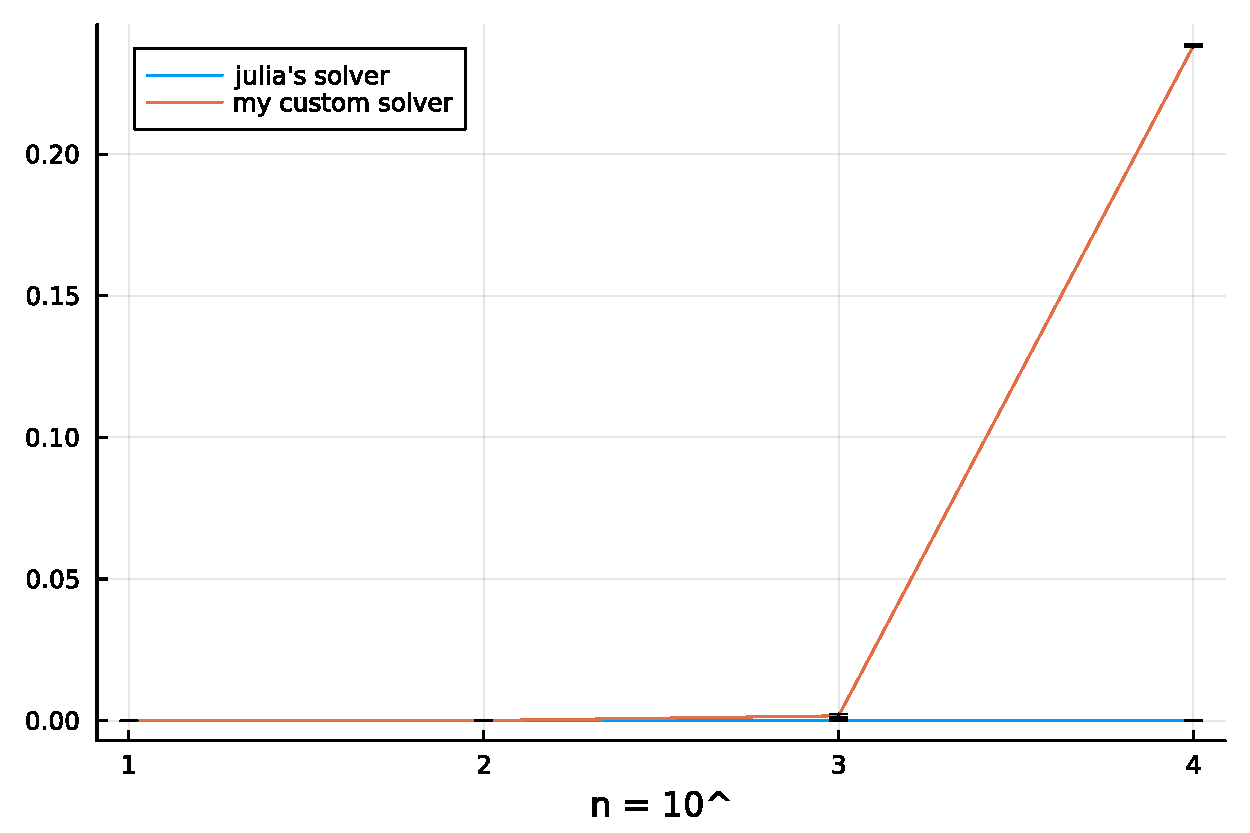
\includegraphics[width=.7\textwidth]{code/q2-1.pdf}
		\end{center}
	\item \textbf{Code}
		\begin{lstlisting}[language=julia]
function solve(A, b)
	L, U, p = lu(A)
	return backsolve(U, forwardsolve(L, b[p]))
end

sol_mean = []
sol_std = []
opt_mean = []
opt_std = []
for n_pow in 1:4
	local n = 10^n_pow
	local sol_time = []
	local opt_time = []
	for n_trial in 1:n_trials
	 	global A = rand(n, n)
	 	global b = rand(n)
	
		@assert norm(A\b - solve(A, b)) < tol
		push!(opt_time, @belapsed A\b)
		push!(sol_time, @belapsed solve(A, b))
	end
	push!(opt_mean, mean(opt_time))
	push!(opt_std, std(opt_time))
	push!(sol_mean, mean(sol_time))
	push!(sol_std, std(sol_time))
end

plot(opt_mean, err=opt_std, label="julia's solver")
p = plot!(sol_mean, err=sol_std, label="my custom solver", xlabel="n = 10^")
		\end{lstlisting}
		\paragraph{Output}
		\begin{center}
			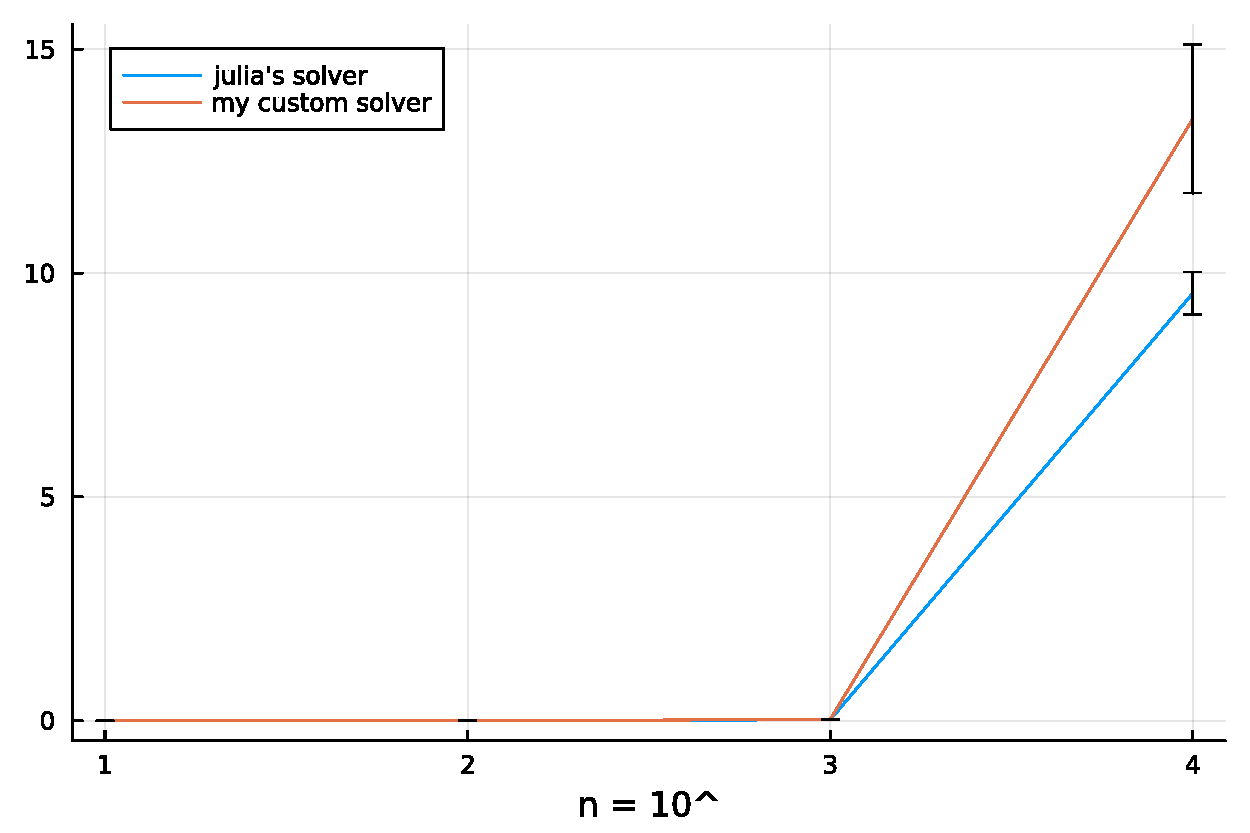
\includegraphics[width=.7\textwidth]{code/q2-2.pdf}
		\end{center}
		Regarding accuracy, we check within the code that the solution obtained by our solver is within tolerance of the optimal solution. Although our naive solution leverages sparse computation, it doesn't beat Julia's optimizations.
\end{enumerate}

\newpage
\question
\hfill

Let $\mM \in \mathbb{R}^{n \times n}$ and $\vx, \vb \in \mathbb{R}^n$. We have:
\begin{equation*}
	\mM \vx = \bmat{\mA & \mB \\ \mC & \mD} \bmat{\vx_1 \\ \vx_2} = \bmat{\vb_1 \\ \vb_2} = \vb
\end{equation*}
With $\vx_1 \in \mathbb{R}^d$ known for some $d \leq n$.

\begin{enumerate}[label=\arabic*.]
	\item Let's merge matrices:
		\begin{gather*}
			\mathrm{Let~} \mY := \bmat{\mA \\ \mC} \quad \mathrm{and} \quad \mZ := \bmat{\mB \\ \mD}
		\end{gather*}
		We now have:
		\begin{align*}
			\mM \vx = \bmat{\mY & \mZ} \bmat{\vx_1 \\ \vx_2} &= \bmat{\vb_1 \\ \vb_2} \\
			\mY \vx_1 + \mZ \vx_2 &= \vb \\
			\mZ \vx_2 &= \vb - \mY \vx_1 \\
			\intertext{Here, we apply the pseudoinverse on both sides:}
			\mZ \mZ^{\dagger} \mZ \vx_2 &= \mZ \mZ^{\dagger} (\vb - \mY \vx_1) \\
			\vx_2 &= \mZ \mZ^{\dagger} (\vb - \mY \vx_1)
		\end{align*}
		The key assumption here is the existence of the pseudoinverse $\mZ^{\dagger}$.
	\item We can perform a similar operation to obtain $\vx_1$ given $\vx_2$:
		\begin{align*}
			\mM \vx = \bmat{\mY & \mZ} \bmat{\vx_1 \\ \vx_2} &= \bmat{\vb_1 \\ \vb_2} \\
			\mY \vx_1 + \mZ \vx_2 &= \vb \\
			\mY \vx_1 &= \vb - \mZ \vx_2 \\
			\mY \mY^{\dagger} \mY \vx_1 &= \mY \mY^{\dagger} (\vb - \mZ \vx_2) \\
			\vx_1 &= \mY \mY^{\dagger} (\vb - \mZ \vx_2)
		\end{align*}
		Like earlier, we assume the existence of $\mY^\dagger$.
	\item The goal is to reduce the system of equations. Unravelling block notation renders two linear systems:
		\begin{gather*}
			\mA \vx_1 + \mB \vx_2 = \vb_1 \quad \mathrm{and} \quad \mC \vx_1 + \mD \vx_2 = \vb_2
		\end{gather*}
		The main idea is to rewrite $\vx_2$ as a function of $\vx_1$ (which is known). We now want just one linear system rather than two.
		The first equation can be rewritten:
		\begin{gather*}
			\mA \vx_1 + \mB \vx_2 = \vb_1 \iff \mA \vx_1 = \vb_1 - \mB \vx_2 \iff \vx_1 = \mA^{-1} (\vb_1 - \mB \vx_2)
		\end{gather*}
		We can plug $\vx_1$ into the second equation:
		\begin{align*}
			\mC \vx_1 + \mD \vx_2 = \vb_2 &\iff \mC \mA^{-1} (\vb_1 - \mB \vx_2) + \mD \vx_2 = \vb_2 \\
			&\iff \mC \mA^{-1} \vb_1 - \mC \mA^{-1} \mB \vx_2 + \mD \vx_2 = \vb_2 \\
			\mC \vx_1 + \mD \vx_2 = \vb_2 &\iff \underbrace{(\mC \mA^{-1} \mB - \mD)}_{\in \mathbb{R}^{(n - d) \times (n - d)}} \vx_2 = \mC \mA^{-1} \vb_1 - \vb_2
		\end{align*}
		Thus, assuming $\mA^{-1}$ exists, we can reduce our system of equations to one in $(n - d) \times (n - d)$, and we can ignore $\vx_1$ as that is already solved. We can borrow from our solver from the previous question to solve for $\vx_2$ efficiently. We can also go in the other direction, and use $\mC^{-1}$ instead. So if one inverse exists but not the other, it should still be possible to simplify computation.
\end{enumerate}

\newpage
\question
\hfill

\begin{enumerate}[label=\arabic*.]
	\item Assuming partial pivots are provided in the format of sparse matrices. \textbf{Code}
		\begin{lstlisting}[language=julia]
function check_lu(A, L, U, p, tol)
	@assert all(diag(L) .== 1)  #  check if L has a diagonal of 1
	@assert tril(L) == L  # check if L is lower triangular
	@assert triu(U) == U  # check if U is upper triangular
	@assert sort(p) == 1:length(p)   # check if it's actually a permutation

	@assert norm(A[p, :] - L * U) < tol  # check reconstruction
end
		\end{lstlisting}
	\item \textbf{Code}
		\begin{lstlisting}[language=julia]
using Plots

A = [2 1 ; 1 2]
b = [5.5 ; 0.5]

function f(A, b, x)
	return x' * A * x / 2 .- x' * b
end

n = 1000
max = 10
min = -10
U = zeros(n, n)

for (idx_i, val_i) in enumerate(range(min, max, length=n))
	for (idx_j, val_j) in enumerate(range(min, max, length=n))
		U[idx_i, idx_j] = f(A, b, [val_i ; val_j])
	end
end

p = surface(U, camera=(40, 60))
		\end{lstlisting}
		\paragraph{Output}
		\begin{center}
			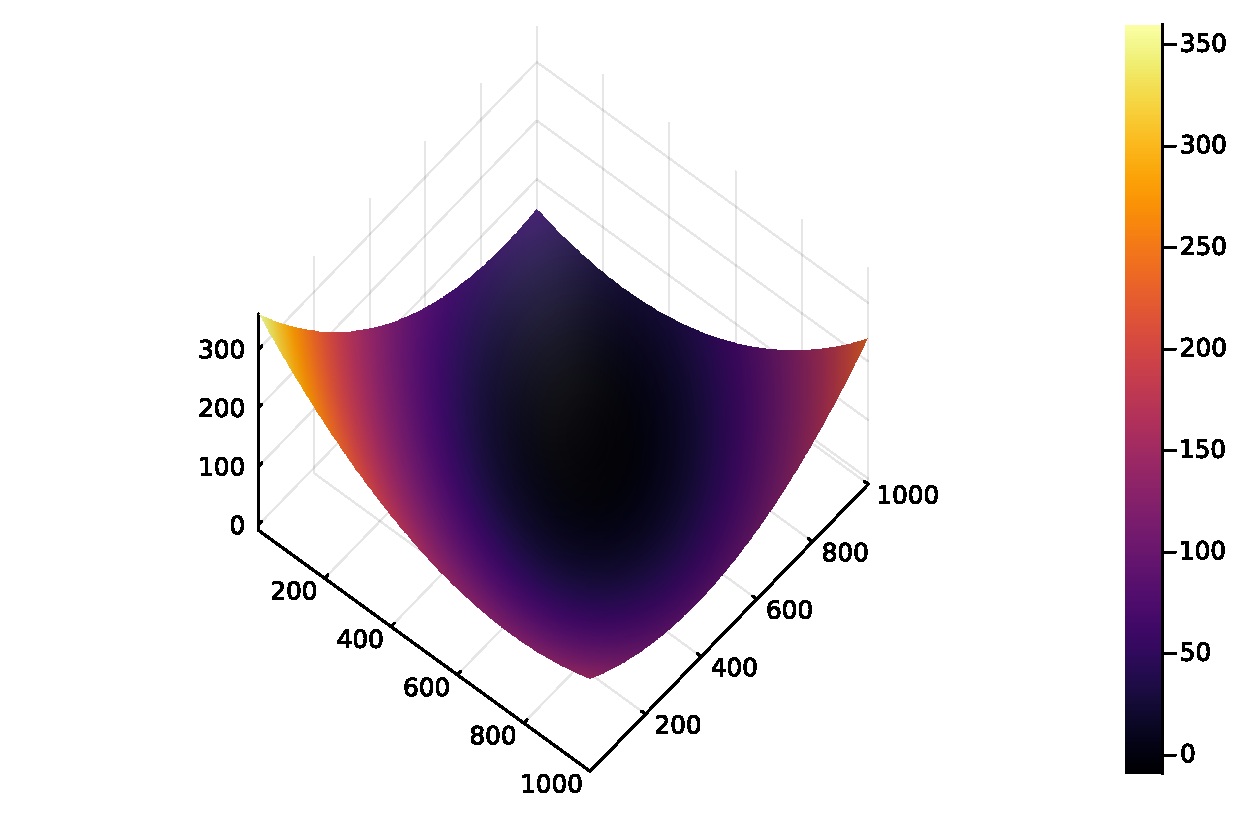
\includegraphics[width=.7\textwidth]{code/q4-1.pdf}
		\end{center}
		Next, we can eliminate a variable.
		\begin{gather*}
			\bmat{2 & 1 \\ 1 & 2} \bmat{\vx_1 \\ \vx_2} = \bmat{5.5 \\ 0.5} \\
			2 \vx_1 + \vx_2 = 5.5 \iff \vx_1 = \frac{5.5 - \vx_2}{2} \\
			\therefore \vx_1 + 2 \vx_2 = 0.5 \iff \frac{5.5 - \vx_2}{2} + 2 \vx_2 = 0.5 \iff 5.5 - \vx_2 + 4 \vx_2 = 1 \iff 4\vx_2 = -4.5
		\end{gather*}
		Thus $\mA' = 4$, $\vb = -4.5$ eliminates $\vx_1$. We can plot this:
		\paragraph{Code}
		\begin{lstlisting}[language=julia]
A = [4]
b = [-4.5]

u = zeros(n)
for (idx_i, val_i) in enumerate(range(min, max, length=n))
	u[idx_i] = f(A, b, [val_i])[1]
end

p = plot(u)
		\end{lstlisting}
		\paragraph{Output}
		\begin{center}
			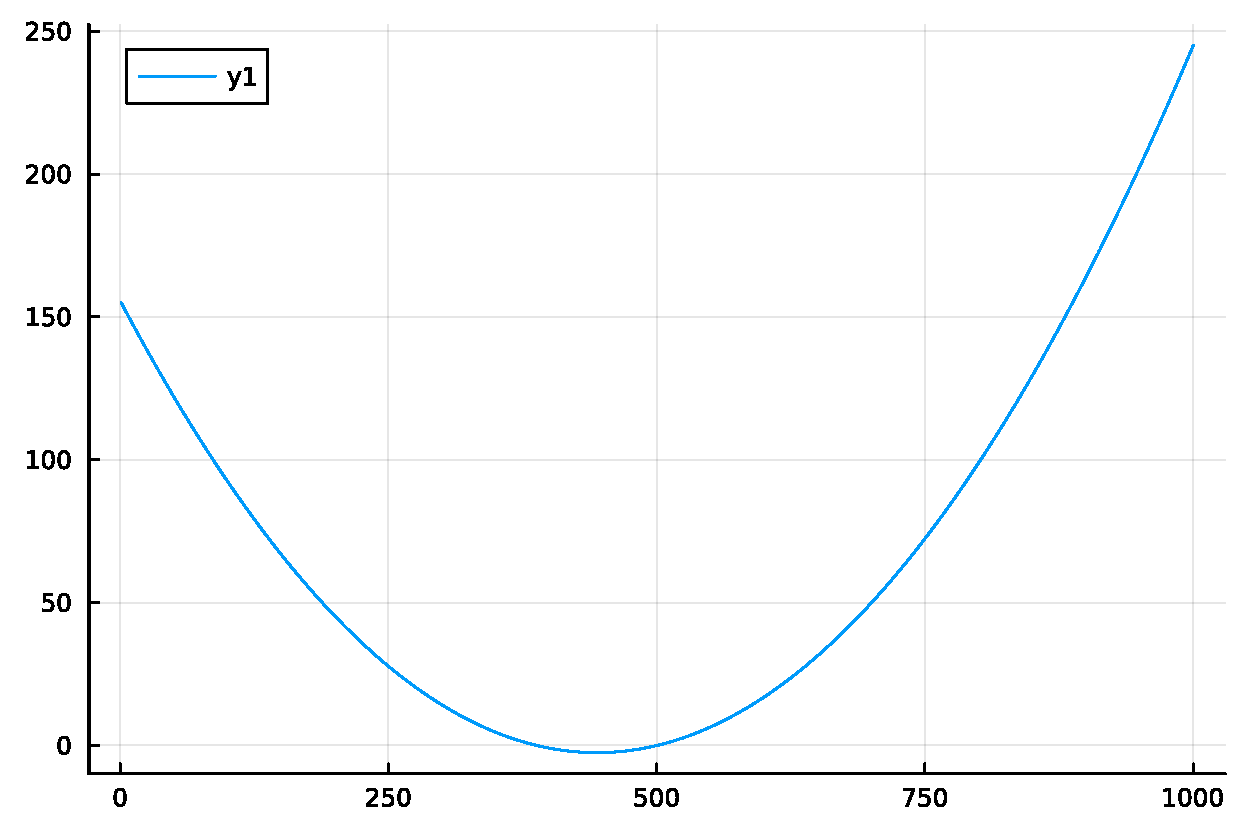
\includegraphics[width=.7\textwidth]{code/q4-2.pdf}
		\end{center}
	\item We have:
		\begin{gather*}
			\mA_{ij} = \begin{cases}
				1 & i = j \\
				-1 & i = j + 1  \\
				0 & \mathrm{otherwise} \\
			\end{cases} \qquad \forall i, j \in \{1, 2, \ldots, n \} \\ 
			\mathrm{Now,~let~} \mX_{ij} := \begin{cases}
				1 & j \geq i \\
				0 & \mathrm{otherwise}
			\end{cases} \qquad \forall i, j \in \{1, 2, \ldots, n\}
		\end{gather*}
		We can then show that $\mA \mX = \mI$ and $\mX \mA = \mI$. The overall strategy is simple, we exclude all the zero-valued indices for each case and compute the resulting value. In particular, we will show that $\mY_{i,j} = 0$ if $i \neq j$ and $1$ if $i = j$ for $\mY = \mX \mA$ and $\mY = \mA \mX$, and $\mY$ is the identity matrix $\mI$.
		\paragraph{Case 1.} $\mA \mX = \mI$. Consider indices $i, j \in \{1, 2, \ldots, n\}$:
		\begin{enumerate}[label=\alph*.]
			\item \textbf{Case a:} $i = j$
				\begin{gather*}
					(\mA \mX)_{ii} = \langle \mA_{i, :}, \mX_{:, i} \rangle = \sum^n_{k = 1} \mA_{ik} \mX_{ki} = \mA_{ii} \mX_{ii} + \mA_{i, i - 1} \mX_{i - 1, i} + 0 = 1 \cdot 1 + -1 \cdot 0 + 0 = 1
				\end{gather*}
			\item \textbf{Case b:} $i < j$
				\begin{gather*}
					(\mA \mX)_{ij} = \langle \mA_{i, :}, \mX_{:, j} \rangle = \sum^n_{k = 1} \mA_{ik} \mX_{kj} = \mA_{ii} \mX_{ij} + \mA_{i,i - 1} \mX_{i-1,j} = 0 + 0 = 0
				\end{gather*}
			\item \textbf{Case c:} $i > j$
				\begin{gather*}
					(\mA \mX)_{ij} = \langle \mA_{i, :}, \mX_{:, j} \rangle = \sum^n_{k = 1} \mA_{ik} \mX_{kj} = \mA_{ii} \mX_{ij} + \mA_{i,i - 1} \mX_{i-1,j} = 1 - 1 = 0
				\end{gather*}
		\end{enumerate}
		\paragraph{Case 2.} $\mX \mA = \mI$
		\begin{enumerate}[label=\alph*.]
			\item \textbf{Case a:} $i = j$
				\begin{gather*}
					(\mX \mA)_{ii} = \langle \mX_{i, :}, \mA_{:, i} \rangle = \sum^n_{k = 1} \mX_{ik} \mA_{ki} = \sum^{i}_{k = 1} \mA_{ki} = \sum^{i-1}_{k=1} 0 + \mA_{ii} = 0 + 1 = 1
				\end{gather*}
			\item \textbf{Case b:} $i < j$
				\begin{gather*}
					(\mX \mA)_{ij} = \langle \mX_{i, :}, \mA_{:, j} \rangle = \sum^n_{k = 1} \mX_{ik} \mA_{kj} = \sum^{i}_{k = 1} \mA_{kj} = 0
				\end{gather*}
			\item \textbf{Case c:} $i > j$
				\begin{gather*}
					(\mX \mA)_{ij} = \langle \mX_{i, :}, \mA_{:, j} \rangle = \sum^n_{k = 1} \mX_{ik} \mA_{kj} = \sum^{i}_{k = 1} \mA_{kj} = \mA_{j-1, j} + \mA_{jj} + 0 = -1 + 1 = 0
				\end{gather*}
		\end{enumerate}
		Since we have that $\mA \mX = \mX \mA = \mI$, we have found a generalized form of the inverse as $\mA^{-1} = \mX$ for arbitrary $n \in \mathbb{N}$.
\end{enumerate}

\end{questions}
\end{document}
